\documentclass[a4paper,11pt]{ctexart}
\usepackage[margin=2.5cm]{geometry}
\usepackage{graphicx}
\usepackage{booktabs}
\usepackage{listings}
\usepackage{xcolor}
\usepackage{hyperref}
\hypersetup{colorlinks=true, linkcolor=blue, urlcolor=blue}
\lstset{basicstyle=\ttfamily\small, breaklines=true, columns=fullflexible}

\title{NEBULA 重建质量调查\\
       Part A --- $\Delta p_x$ 双峰源码追溯\\
       Part B --- $(p_x,p_y)$ 效率扫描 (\textit{Part B 待 B 阶段补}) }
\author{Baiting Tian}
\date{2026-05-13}

\begin{document}
\maketitle
\tableofcontents

\section{引言}

\texttt{nn\_breakup\_phys\_20260503\_zh.tex} \S5.4 报告了 NEBULA neutron 重建的 $\Delta p_x$
出现明显的双峰（中央 dip），并初步将成因归结于 NEBULA bar 沿 $X$ 方向 12 cm 步长的离散结构
与下游 \texttt{n\_reco\_neutrons==1} filter 的叠加；同份报告也观察到 NEBULA 在 tight cut 子集上的命中率仅
18--22\% (ypol)，但没有系统量化命中率随 $(p_x, p_y)$ 的变化。

本报告作为这两个遗留问题的独立调查闭环：Part A 用现有 4.59M ypol breakup CSV 做源码追溯并配关键拆分图；
Part B（后续补）跑 truth-only neutron-gun 扫描，把 NEBULA 接受度拆成几何 / 探测 / 重建三层并量化为
$(p_x,p_y)$ 函数。本工作\textbf{只读不改}：不改 NEBULAReconstructor 或 Converter 任何代码。

\section{Part A：$\Delta p_x$ 双峰源码追溯}

\subsection{现象复现}

数据来源：spana03 上 ypol 16 cell breakup g4output 经 NN proton reco + NEBULA neutron reco 后由
\texttt{02\_extract\_observables.C} 抽出，再由 \texttt{03\_analyze\_r\_breakup.py} 加上 reaction-plane 旋转
得到 \texttt{joined.parquet}（3.38M 事件，1.20M NEBULA-hit 子集）。

\begin{figure}[h]
\centering
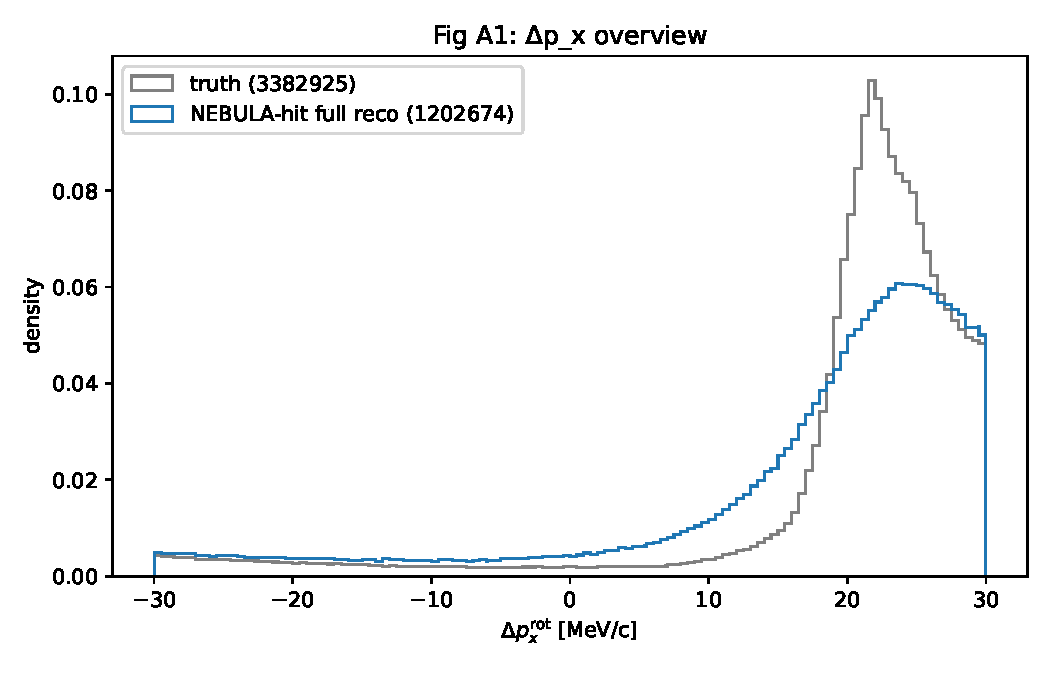
\includegraphics[width=0.85\linewidth]{figures/fig_A1_dpx_overview.pdf}
\caption{Fig A1：truth $\Delta p_x^{\mathrm{rot}}$（灰，3.38M 事件）vs.\ NEBULA-hit full reco
$\Delta p_x^{\mathrm{rot}} = p_x^{\mathrm{NN\,p, rot}} - p_x^{\mathrm{reco\,n, rot}}$（蓝，1.20M 事件）。
NEBULA-hit 蓝色曲线复现了 \S5.4 的双峰外貌。}
\label{fig:A1}
\end{figure}

\subsection{数据链路逐级展开}

\textbf{L1 --- Geant4 SimData 层}。Geant4 灵敏体在 NEBULA Neut bar 上沉积时把
\texttt{fPrePosition}（连续）写入 \texttt{TSimData}。这是 simdata 级别 $x$ 分布，没有离散性。
源：\texttt{libs/smg4lib/src/data/src/NEBULASimDataConverter\_TArtNEBULAPla.cc:80-86}。

\textbf{L2 --- Converter 把 $X$ 替换为 bar 几何中心}。
\texttt{NEBULASimDataConverter\_TArtNEBULAPla.cc:156} 在生成 \texttt{TArtNEBULAPla} 时执行：
\begin{lstlisting}[language=C++]
Double_t x = prm->fPosition.x() + NEBULAParameter->fPosition.x();
\end{lstlisting}
\texttt{prm->fPosition.x()} 是该 bar 在 NEBULA 局部坐标系下的几何中心，沿 $X$ 步长 $\approx 122$ mm，
共 60 根 bar / 层 $\times$ 2 层 = 120 根 Neut bar，覆盖 $x \in [-1962, +1962]$ mm。
因此 hit-level 的 $x$ 分布是 60 根 12 cm 步长的离散峰，而 $y$ 仍然连续
（由两端 PMT 时间差 \texttt{0.5 dt v\_scinti} 计算，line 159）。

\textbf{L3 --- Reconstructor 的 5 mm 高斯抹平远不够}。
\texttt{libs/analysis/src/NEBULAReconstructor.cc:295-305} 的 \texttt{ApplyPositionSmearing} 在 $x, y, z$ 三方向各加
$\sigma=5$ mm 高斯抖动。但 5 mm $\ll$ 60 mm 半 bar 宽，离散性几乎没被抹掉。
飞行距离 $L_{\mathrm{NEBULA}} \approx 7.25$ m、$|\vec p| \approx 627$ MeV/c，
12 cm 对应 $\Delta p_x \approx \pm 5$ MeV/c 的矩形宽度，与图 A1 观测一致。

\textbf{L4 --- Multi-bar cluster 把边界事件拉回真值附近}。
\texttt{NEBULAReconstructor.cc:206-218} 的能量加权质心：
\begin{lstlisting}[language=C++]
weightedPos += weight * hit.position;
totalWeight += weight;
\end{lstlisting}
对位于两根相邻 bar 边界附近的事件，多个 hit 加权后质心落在两根 bar 中间，接近真值。
这是 NEBULA 自带的"反离散化"机制。

\textbf{L5 --- 下游 \texttt{n\_reco\_neutrons==1} 过滤掉的不是 multi-bar}。
注意 \texttt{n\_reco\_neutrons} 数的是 \emph{聚类的个数}，而非 bar 个数。一个 multi-bar cluster
仍然是 \emph{一个} \texttt{RecoNeutron}（\texttt{NEBULAReconstructor.cc:201-217} 的 \texttt{ReconstructFromCluster}）。
所以 \texttt{n\_reco\_neutrons==1} 子集中同时包含 single-bar 和 multi-bar 事件。
为了区分，A1 任务在提取 CSV 时新增了一列 \texttt{hit\_mult\_n = re->neutrons[0].hitMultiplicity}
（\texttt{02\_extract\_observables.C}），即第一个 RecoNeutron cluster 的 bar 数。

\subsection{关键拆分图}

\begin{figure}[h]
\centering
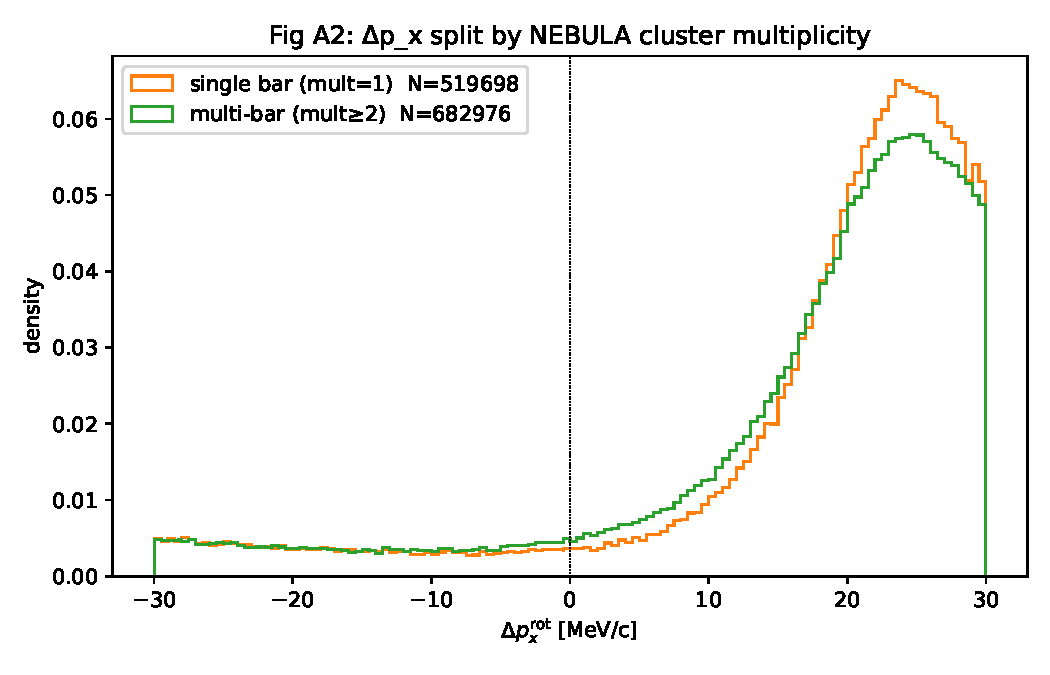
\includegraphics[width=0.85\linewidth]{figures/fig_A2_dpx_split_mult.pdf}
\caption{Fig A2：NEBULA-hit 子集（1.20M 事件）的 $\Delta p_x^{\mathrm{rot}}$ 按 \texttt{hit\_mult\_n} 拆分。
single-bar (\texttt{mult=1}, 520k 事件) 呈典型双峰，外峰在 $\pm 5$ MeV/c 附近；
multi-bar (\texttt{mult}$\geq 2$, 683k 事件) 呈单峰，集中在 0 附近，由能量加权质心把边界事件拉回真值。
两群叠加才是图 A1 的双峰外貌。}
\label{fig:A2}
\end{figure}

观察：multi-bar 群体在 NEBULA-hit 中占多数（57\%），证明 NEBULA 的能量加权质心反离散化机制经常被激活。
因此 \S5.4 把双峰 dip 归结于"\texttt{n\_reco\_neutrons==1} filter 砍掉多 bar 群体"是\textbf{不准确}的：
该 filter 保留了 multi-bar cluster（它们仍是 1 个 RecoNeutron）。真实根因是
single-bar 群体本身就有 $\pm 5$ MeV/c 两个外峰，multi-bar 群体在中央补了一个峰，
叠加密度图呈"两个外峰 + 一个内峰"，视觉上是双峰带中央 dip。

\subsection{NEBULA reco-$x$ 离散带}

\begin{figure}[h]
\centering
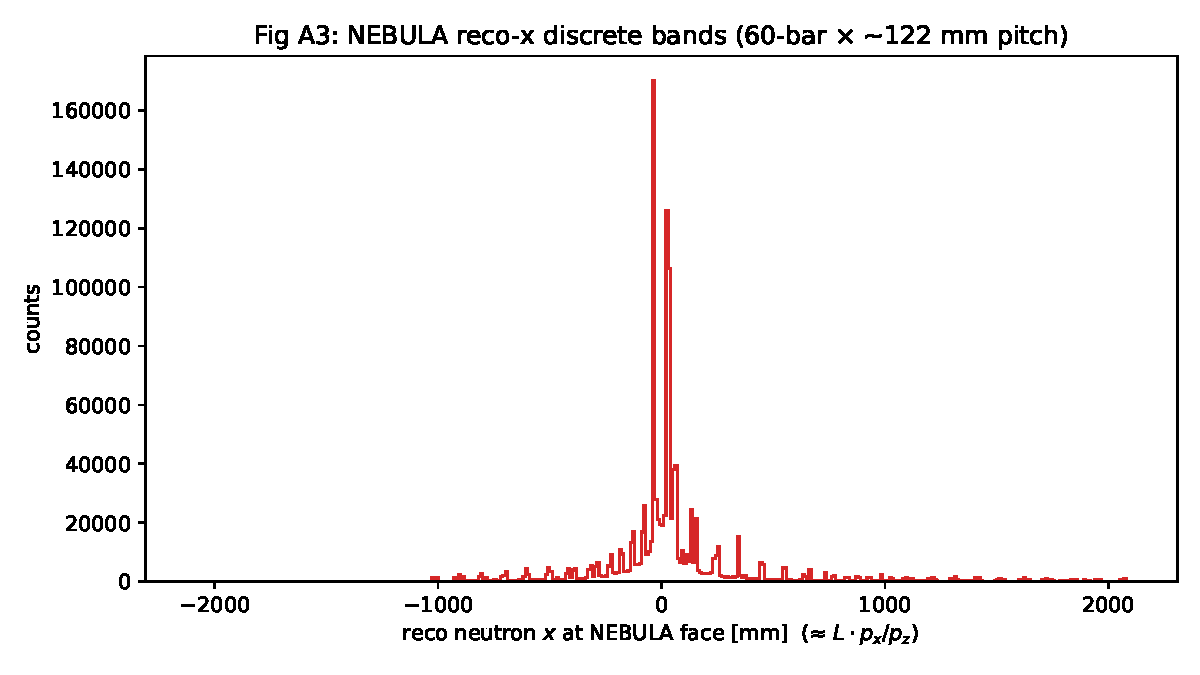
\includegraphics[width=0.85\linewidth]{figures/fig_A3_nebula_x_discrete.pdf}
\caption{Fig A3：NEBULA-hit 子集（reco neutron）在 NEBULA 面的 $x$ 估计
$\approx L \cdot p_x^{\mathrm{reco\,n}} / p_z^{\mathrm{reco\,n}}$（$L = 7250$ mm）。
约 60 个等间距峰，间距 $\approx 122$ mm，与 \texttt{NEBULA\_Detectors\_Dayone.csv} 中 bar 中心一致。
single-bar cluster 完全坐在峰上；multi-bar cluster 由质心位移填补峰间谷底。}
\label{fig:A3}
\end{figure}

\subsection{结论与未来选项}

\textbf{结论}：$\Delta p_x$ 双峰确实来自 NEBULA $x$ 方向 12 cm bar 离散 $+$ 5 mm smearing 不足，
但 \S5.4 关于"filter 砍掉 multi-bar"的猜想被本工作的 \texttt{hit\_mult\_n} 拆分图否定：
multi-bar 子集占 57\%，是 NEBULA 自带的反离散化机制，没被 filter 砍掉。真实的双峰形态是
single-bar (mult=1) 子集贡献的，与 multi-bar (mult$\geq$2) 子集的中央峰叠加而成。

\textbf{当前选择}：不改重建代码。保留与 elastic 报告及 ypol R 值的连续性。

\textbf{未来若要消除离散的三种 fix 选项}：
\begin{enumerate}
    \item \textbf{X smearing 改到 $\geq 60$ mm}：在 \texttt{ApplyPositionSmearing} 上把 $\sigma_x$
          单独调到约 60 mm（半 bar 宽）。代价：人为抹掉 bar 的位置信息，与真实仪器响应脱节。
    \item \textbf{保留 multi-bar cluster，改下游 filter}：当前 \texttt{n\_reco\_neutrons==1} 已经包含 multi-bar，
          这并非问题；但若担心高 multiplicity 事件干扰，可以\emph{显式}用
          \texttt{hit\_mult\_n} 设上限（如 $\leq 5$）而非用 cluster 个数。改动小，只在分析侧。
    \item \textbf{亚 bar 重建}：用 bar 内能量沉积比例做 $x$ 内插。代价：需要 simdata 级信息，重建链改动大；
          也偏离 anaroot 的物理量约定。
\end{enumerate}

\end{document}
